\begin{graphicspathcontext}{{./chapters/simulation/imgs/},{./chapters/simulation/imgs/auto/},\old}

\begin{frame}{{Several Definitions} of Simulation}
	\begin{definitionblock}{\cite{Shannon77}}
		The process of \Emph{designing a model} of a real system and \Emph{conducting experiments } with this model for the purpose either of \Emph{understanding} the behavior of the system or of \Emph{evaluating} various strategies (within the limits imposed by a criterion or a set of criteria) for the operation of the system.
	\end{definitionblock}
	\vspace{.5cm}
	\begin{definitionblock}{\cite{Fishwick97}}
		Computer simulation is the discipline of designing a model of an actual or theoritical physical system, executing the model on a digital computer, and analyzing the execution output.
	\end{definitionblock}
\end{frame}

\sidenote{Image Claude Sonnet 4.6}
\figureslide{{Standard Lifecycle} of a Simulation Model}{simulation_lifecycle}

\sidecite{Zeigler00}
\figureslide{Relation between the real system and the simulation model}{simulation_basics}

\sidecite{Zeigler00}
\begin{frame}[t]{{Modeling Relation:} System $\leftrightarrow$ Model}
	\begin{center}
		\includegraphics[width=.8\linewidth]{system_model_relation}
	\end{center}
	\vspace{.5cm}
	\begin{itemize}
	\item To determine if the system model is an acceptable simplificiation in terms of quality criteria and experimentation objectives.
	\item Directly related to the consistency of the model simulation.
	\end{itemize}
\end{frame}

\sidecite{Zeigler00}
\begin{frame}[t]{{Simulation Relation:} Model $\leftrightarrow$ Simulator}
	\begin{center}
		\includegraphics[width=.8\linewidth]{model_simulator_relation}
	\end{center}
	\vspace{.5cm}
	\begin{itemize}
	\item To guarantee that the simulator, used to implement the model, correctly generates the behavior of the model.
	\item To be sure that the simulator reproduces clearly the mechanisms of change of state are formalized in the model.
	\end{itemize}
\end{frame}

\sidenote{Images Claude Sonnet 4.6}
\begin{frame}[t]{What is simulated?}
	\begin{columns}
		\begin{column}[t]{.5\linewidth}
			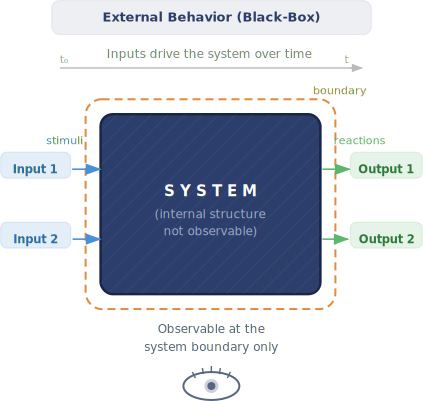
\includegraphics{simulation_external_behavior}
		\end{column}
		\begin{column}[t]{.5\linewidth}
			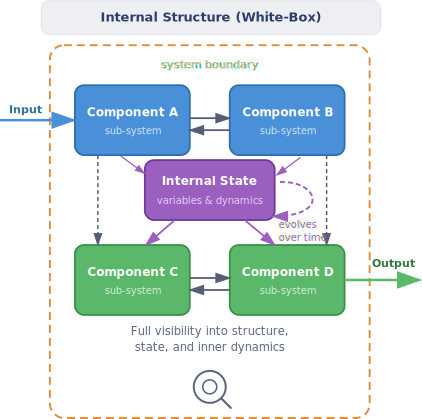
\includegraphics{simulation_internal_structure}
		\end{column}
	\end{columns}
\end{frame}

\begin{frame}[t]{{System Dynamic:} Defining the Time Advance Function}
	\vspace{-.5cm}
	\begin{columns}
		\begin{column}[t]{.2\linewidth}
			\begin{bottomarrowsequence}
				\only<1>{\arrow[bg=CIADgreen]{Continuous Time}}
				\only<2->{\arrow{Continuous Time}}
				\only<1,3>{\arrow{Discrete Time}}
				\only<2>{\arrow[bg=CIADgreen]{Discrete Time}}
				\only<1-2>{\arrow{\ahc{Event-based}{Time}}}
				\only<3>{\arrow[bg=CIADgreen]{\ahc{Event-based}{Time}}}
			\end{bottomarrowsequence}
		\end{column}
		\begin{column}[t]{.8\linewidth}
			\only<1>{
				\smaller
				\begin{block}{Principle}
					\begin{compactitemize}
						\item Time $t \in \mathbb{R}_{\geq 0}$ flows \emph{continuously} and without interruption
						\item The system state $\mathbf{x}(t)$ is defined at \emph{every} instant $t$
						\item The dynamics are governed by a system of \Emph{ordinary differential equations}
					\end{compactitemize}
				\end{block}
				\begin{block}{Mathematical Model}
					\begin{compactdescription}
					\item[State Evolution] $\frac{d\,\mathbf{x}(t)}{dt} = f\!\bigl(\mathbf{x}(t),\,\mathbf{u}(t),\,t\bigr), \quad \mathbf{x}(t_0) = \mathbf{x}_0$
					\item[Output] $\mathbf{y}(t) = g\!\bigl(\mathbf{x}(t),\,\mathbf{u}(t),\,t\bigr)$
					\end{compactdescription}
					where $\mathbf{x}\!\in\!\mathbb{R}^n$ is the state vector, $\mathbf{u}\!\in\!\mathbb{R}^m$ the input, and $\mathbf{y}\!\in\!\mathbb{R}^p$ the output
				\end{block}
				\centering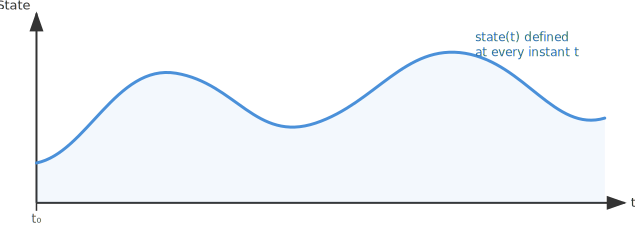
\includegraphics[width=.8\linewidth]{time_continuous}
			}
			\only<2>{
				\smaller
				\begin{block}{Principle}
					\begin{compactitemize}
						\item Time advances in \emph{uniform steps}: $t_k = t_0 + k\,\Delta t, \quad k \in \mathbb{N}$
						\item The system state $\mathbf{x}_k$ is only defined \emph{at the discrete instants} $t_k$
						\item Between two steps, the state is \Emph{not observed}
					\end{compactitemize}
				\end{block}
				\begin{block}{Mathematical Model}
					\begin{compactdescription}
					\item[State Evolution] $\mathbf{x}_{k+1} = f\!\bigl(\mathbf{x}_k,\,\mathbf{u}_k,\,k\bigr), \quad \mathbf{x}_0 \text{ given}$
					\item[Output] $\mathbf{y}_k = g\!\bigl(\mathbf{x}_k,\,\mathbf{u}_k,\,k\bigr)$
					\end{compactdescription}
					where $\mathbf{x}\!\in\!\mathbb{R}^n$ is the state vector, $\mathbf{u}\!\in\!\mathbb{R}^m$ the input, and $\mathbf{y}\!\in\!\mathbb{R}^p$ the output
				\end{block}
				\centering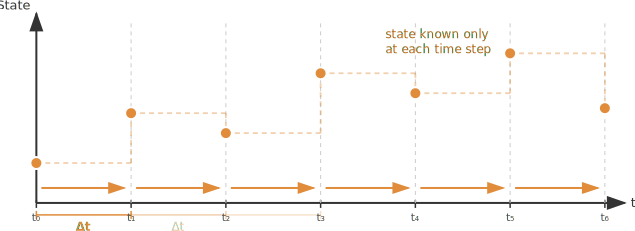
\includegraphics[width=.8\linewidth]{time_discrete_constant}
			}
			\only<3>{
				\smaller
				\begin{block}{Principle}
					\begin{compactitemize}
						\item Time advances \emph{only when an event occurs}
						\item Between two consecutive events, the state is \Emph{constant}
						\item Time steps $\Delta t_k$ are \Emph{variable} and determined by the event schedule
					\end{compactitemize}
				\end{block}
				\begin{block}{Mathematical Model}
					Let $\mathcal{E} = \{e_1, e_2, \ldots\}$ the ordered sequence of events
					\begin{compactdescription}
					\item[Time Advance Evolution] $\Delta t_k = t_{k+1} - t_k > 0$
					\item[State transition at event $e_k$] $\mathbf{x}(t_k+1) = \delta\!\bigl(\mathbf{x}(t_k),\, e_k\bigr)$
					\end{compactdescription}
				\end{block}
				\centering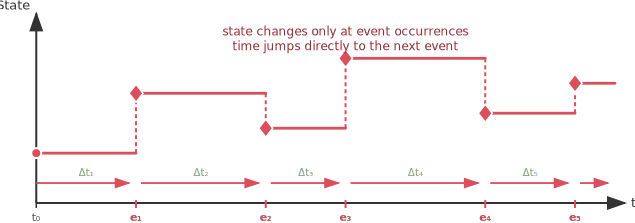
\includegraphics[width=.8\linewidth]{time_event_based}
      			}
		\end{column}
	\end{columns}
\end{frame}

\sidenote{\cite{Hoogendoorn01, Davidsson00}, Image Claude Sonnet 4.6}
\figureslide{{Standard Scales} of Simulation Models}{simulation_model_scales}

\begin{frame}{{Macroscopic Model:} Advantages and Disadvantages}
	\hiconbox{
		\begin{compactdescription}
		\item[Low computational cost] few variables, fast execution
		\item[Scalable] to very large systems without additional cost
		\item[Analytically tractable] closed-form solutions often exist
		\item[Simple to calibrate] aggregate data usually available
		\item[Stable] numerical behaviour with well-known solvers
		\end{compactdescription}}{simu-pros-icon}
	\hiconbox{
		\begin{compactdescription}
		\item[Low accuracy] at fine scales individual behaviour is lost
		\item[Cannot capture] local interactions, heterogeneity, or emergent phenomena
		\item[Strong assumptions] required (homogeneity, mean-field, \ldots)
		\item[Poor predictive power] when individual variability matters
		\item[Validation is difficult] when no aggregate ground truth exists
		\end{compactdescription}}{simu-cons-icon}
\end{frame}

\begin{frame}{{Mesoscopic Model:} Advantages and Disadvantages}
	\hiconbox{
		\begin{compactdescription}
		\item[Balanced trade-off] between accuracy and computational cost
		\item[Captures group dynamics] and statistical heterogeneity
		\item[More realistic] than macro without the cost of micro
		\item[Flexible granularity] group size can be tuned
		\item[Compatible] with both macro and micro representations, enabling multilevel coupling
		\end{compactdescription}}{simu-pros-icon}
	\hiconbox{
		\begin{compactdescription}
		\item[More complex] to design and implement than macro models
		\item[Higher cost] than macro, lower accuracy than micro
		\item[Requires statistical data] for calibrating distributions
		\item[Group boundaries] may be arbitrary and hard to justify
		\item[Emergent individual behaviour] not fully captured
		\end{compactdescription}}{simu-cons-icon}
\end{frame}

\begin{frame}{{Microscopic Model:} Advantages and Disadvantages}
	\hiconbox{
		\begin{compactdescription}
		\item[Highest accuracy] individual behaviour fully represented
		\item[Captures emergent phenomena] arising from local interactions
		\item[Heterogeneity] modelled naturally per entity
		\item[No aggregation assumptions] results are more faithful to reality
		\item[Rich observable outputs] individual trajectories available
		\end{compactdescription}}{simu-pros-icon}
	\hiconbox{
		\begin{compactdescription}
		\item[Very high computational cost] scales poorly with system size
		\item[Large memory footprint] one state record per entity
		\item[Hard to calibrate] individual-level data rarely available
		\item[Complex to implement] and to verify
		\item[Results hard to interpret] at the global scale without post-processing aggregation
		\end{compactdescription}}{simu-cons-icon}
\end{frame}

\sidenote{\cite{GallandGaudDemangeKoukam2014_703}, Images Claude Sonnet 4.6}
\begin{frame}[t]{{Multilevel Model:} coupled models or dynamic model}
	\begin{columns}
		\begin{column}{.5\linewidth}
			\centering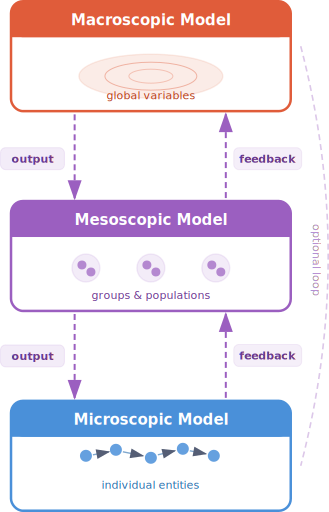
\includegraphics[height=.9\textheight]{multilevel_coupling}
		\end{column}
		\begin{column}{.5\linewidth}
			\centering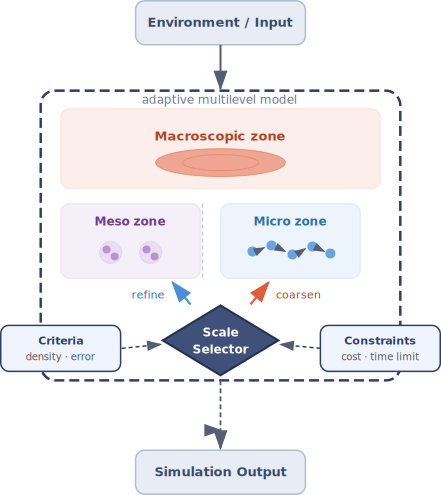
\includegraphics[height=.9\textheight]{multilevel_dynamic}
		\end{column}
	\end{columns}
\end{frame}

\end{graphicspathcontext}

\endinput

